\section{Prototüüp} \label{prototuup}

Käesolev peatükk kirjeldab loodud prototüüpi. Alapeatükis~\ref{prototuup:nouded} esitatakse süsteemile seatud funktsionaalsed ja mittefunktsionaalsed nõuded. Alapeatükk~\ref{prototuup:arhitektuur} kirjeldab süsteemi arhitektuuri. Alapeatükis~\ref{prototuup:tehnoloogiad} põhjendatakse tehnoloogiavalikut. Alapeatükk~\ref{prototuup:liides} kirjeldab kasutajaliidest ning tagasiside esitamise põhimõtteid. Alapeatükis~\ref{prototuup:eetika} käsitletakse süsteemi eetilisi piiranguid ja nende tehnilist realiseerimist.

\subsection{Nõuded} \label{prototuup:nouded}

Funktsionaalsed nõuded olid järgmised. Süsteem peab võimaldama kasutajal (1) sisestada eestikeelse teksti vabavormiliselt, (2) valida peatüki tüübi (sissejuhatus, taust, metoodika, tulemused, kokkuvõte), (3) saada struktureeritud tagasisidet neljas eelmainitud kategoorias, (4) näha iga leiu juures konkreetset probleemset tekstilõiku, soovitust ja kindlushinnangut, (5) valida üldise ja struktureeritud prompti vahel võrdluseks ning (6) eksportida tagasiside tekstifailina.

Mittefunktsionaalsed nõuded olid järgmised. Süsteem peab (1) töötama ühel tüüpilisel arendaja töömasinal ilma erilise riistvara nõudeta, (2) olema kasutatav tavalise veebibrauseri kaudu, (3) vastama tüüpilisele päringule alla 30 sekundi, (4) hoidma kasutaja teksti kogu töö vältel \emph{ainult} mälus ja mitte kettal püsivalt, (5) edastama teksti välimise LLM-i API-ga ainult juhul, kui kasutaja on selle valiku teadlikult kinnitanud, ning (6) võimaldama proovikäivitust ka ilma välise LLM-i API juurdepääsuta (näiteks olukorras, kus hindajal pole API võtit), et töö praktiline tulemus oleks reprodutseeritav minimaalsete eeldustega.

\subsection{Süsteemi arhitektuur} \label{prototuup:arhitektuur}

Prototüüp järgib lihtsat klient-server arhitektuuri. Arhitektuur on kujutatud joonisel~\ref{fig:arhitektuur}. Süsteem koosneb kolmest komponendist: brauseripoolne kasutajaliides (\textbf{frontend}), kohalik teenus (\textbf{backend}) ja välimine LLM-i API. Backend hoiab promptide malle ja vastutab nende sidumise eest sisestatud tekstiga ning JSON-vastuse järeltöötluse eest. Backend on kavandatud kihilisena nii, et LLM-i pakkuja vahetamine (näiteks Anthropic Claude'ilt OpenAI GPT-le) nõuab muutusi ainult \texttt{providers/} kaustas.

Lisaks reaalsetele LLM-pakkujatele on backendis sama liidese taga ka \emph{demo-pakkuja}, mis tagastab iga peatüki tüübi jaoks varem genereeritud salvestatud näidisvastuse (vt fail \texttt{prototuup/backend/demo\_andmed.py}). Demo-pakkuja on vaikevalik, mis võimaldab süsteemi proovida ja töö praktilist tulemust reprodutseerida ilma Anthropici või OpenAI API võtmeta; päris LLM-i kasutamiseks valib kasutaja kasutajaliideses mudeli \texttt{claude-opus-4-7} või \texttt{gpt-5}, mille kasutamine eeldab vastava võtme seadistamist keskkonnamuutujasse.

\begin{figure}[ht]
    \centering
    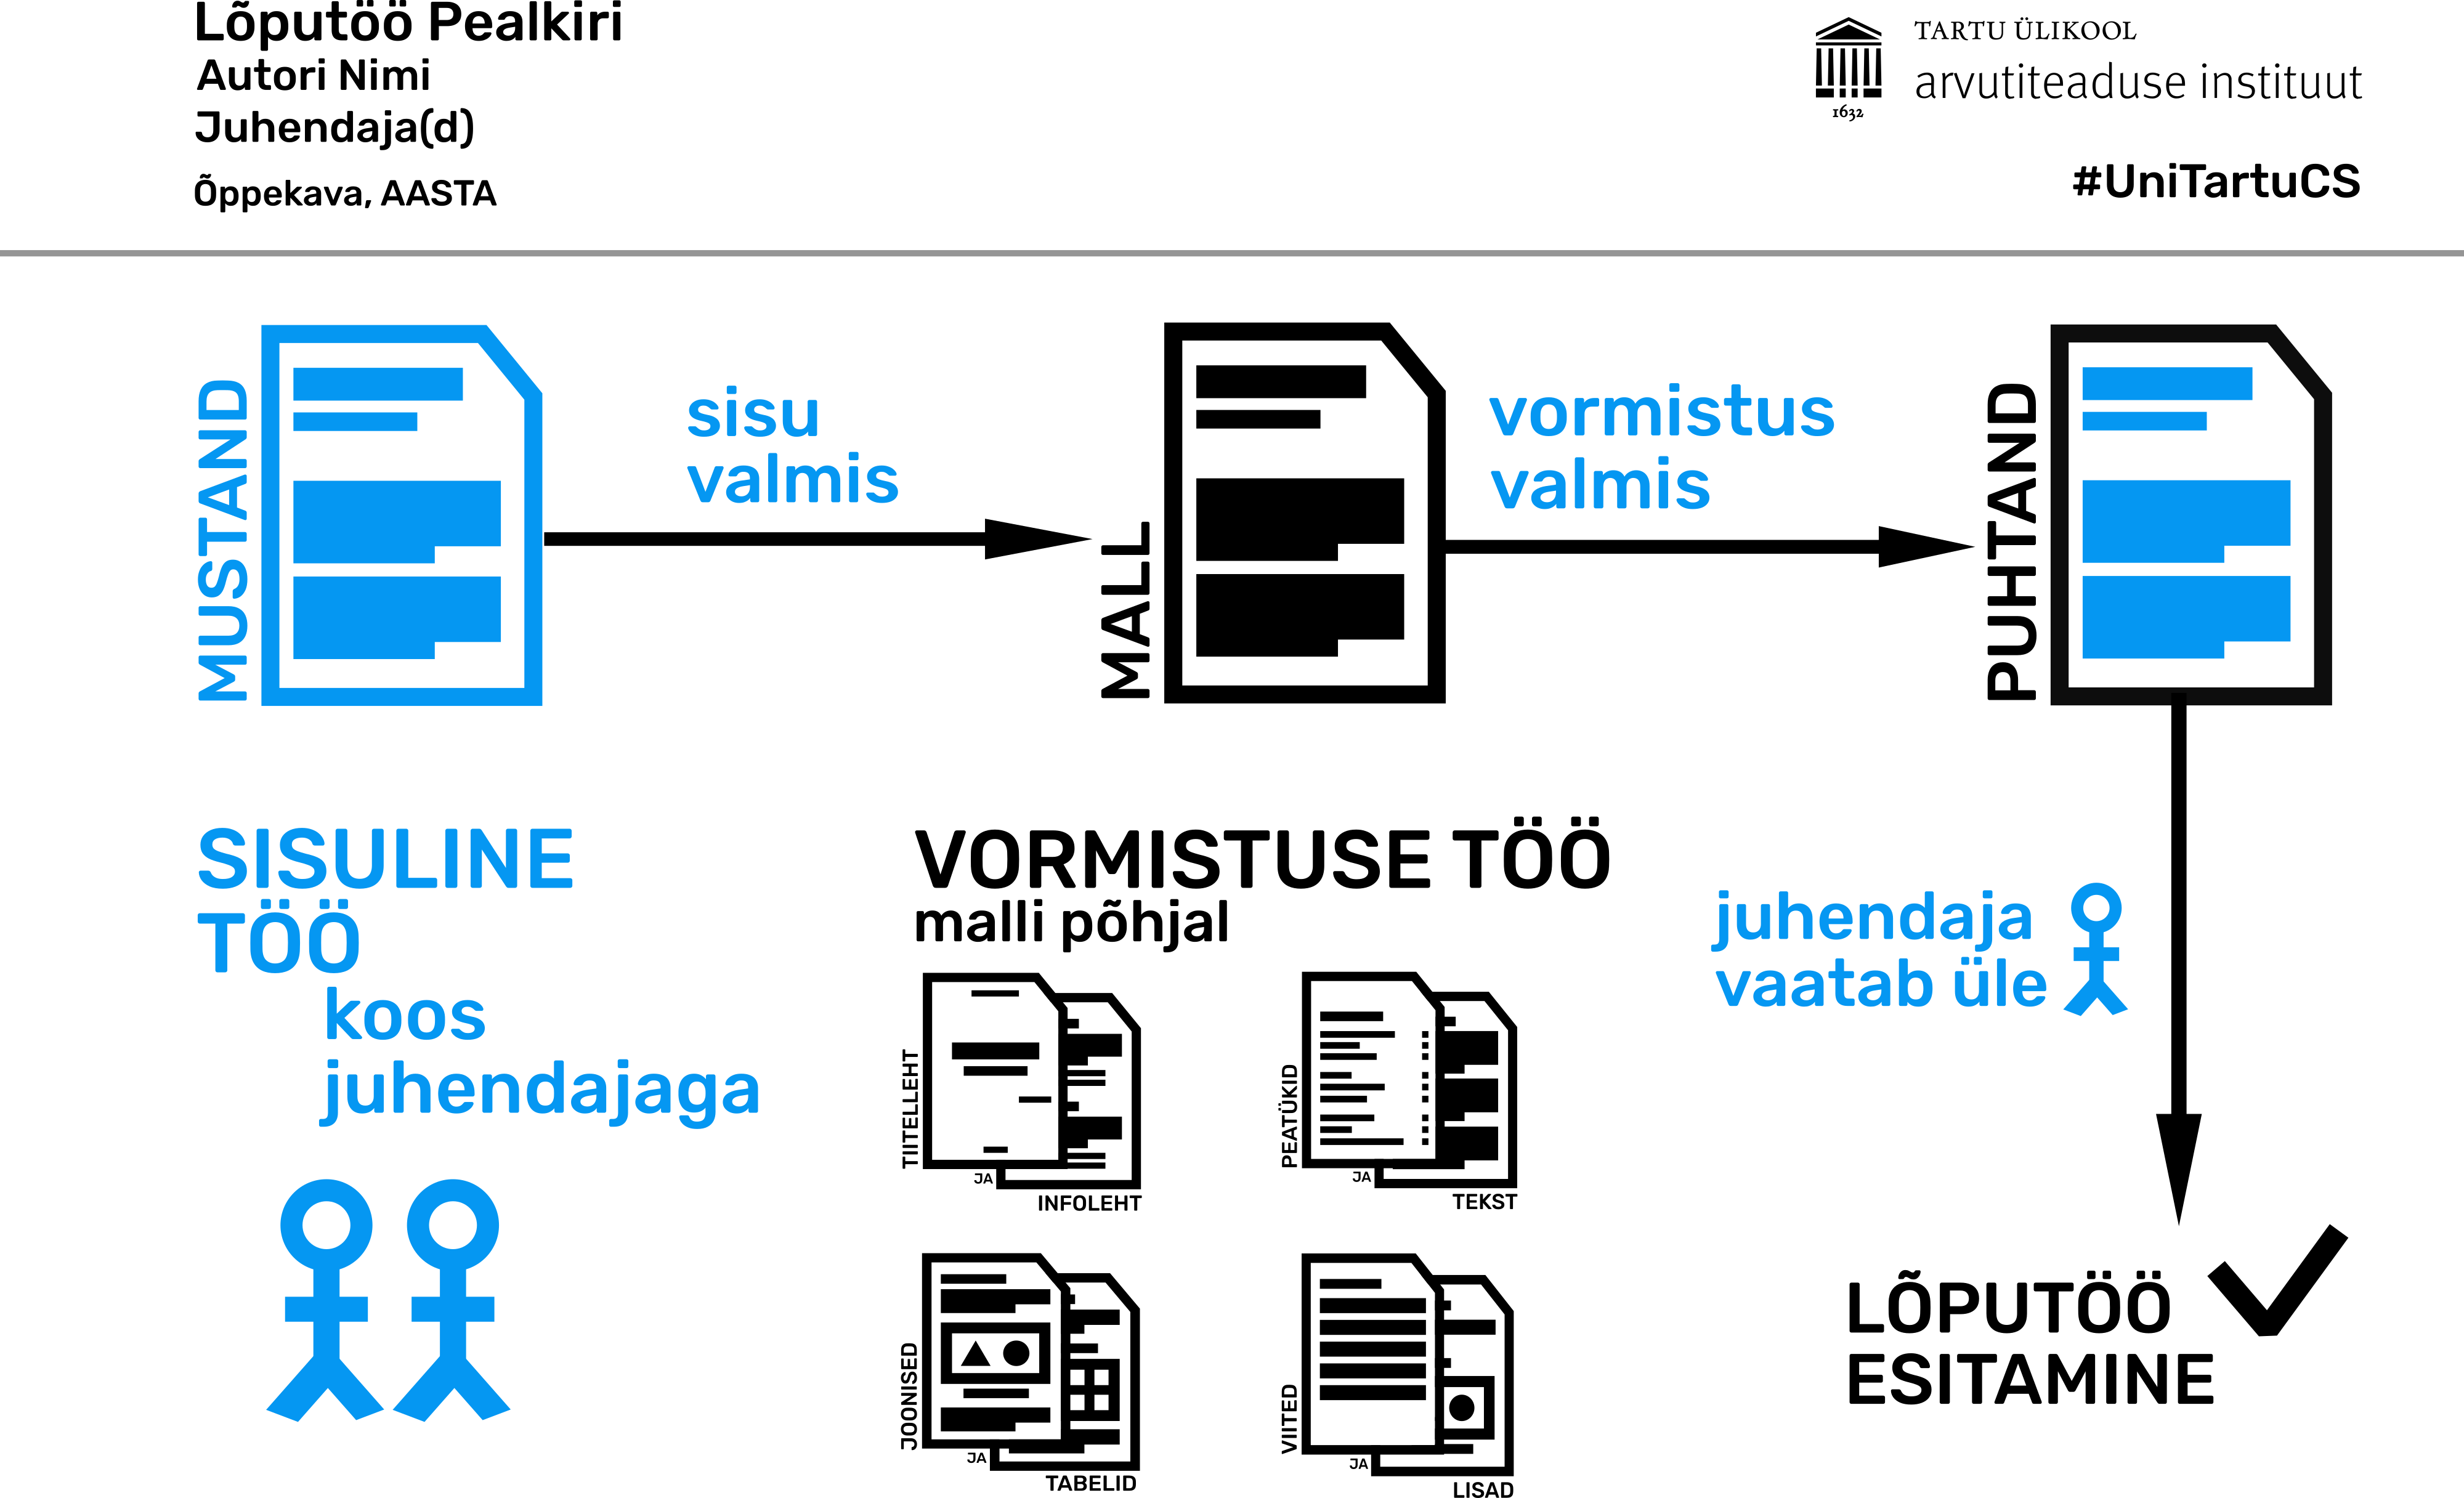
\includegraphics[width=\textwidth]{joonised/Joonis0-VisuaalneKokkuvõte.png}
    \caption{Süsteemi üldine arhitektuur. Kasutaja sisestab teksti veebiliidesesse, mis saadab selle kohaliku backend-teenuse poole. Backend valib valitud prompti malli, kombineerib selle tekstiga ning saadab päringu LLM-i API-le. Mudeli vastus dekodeeritakse JSON-iks, valideeritakse skeemi vastu ning kuvatakse kasutajale.}
    \label{fig:arhitektuur}
\end{figure}

\subsection{Tehnoloogiavalik} \label{prototuup:tehnoloogiad}

Prototüübi realiseerimisel valiti tehnoloogiad järgmiste põhimõtete alusel: tuntud ja levinud tehnoloogiad (et reprodutseeritavus oleks lihtne), minimaalne lisakulu (\emph{ingl. overhead}) ja kiire arendustsükkel.

\begin{table}[htb!]
    \centering
    \caption{Prototüübi tehnoloogiline kombinatsioon ja valiku põhjendus.}
    \label{tab:tehnoloogiad}
    \begin{tblr}{width=1.0\textwidth, hlines, vlines,
                colspec = { Q[l,font=\bfseries,wd=0.20\textwidth] Q[l,wd=0.20\textwidth] X[l] },
                row{1} = {font=\bfseries, bg = colorCellHighlight},
            }
    Komponent & Tehnoloogia & Põhjendus \\
    Backend & Python 3.12 + FastAPI & Anthropic SDK on Pythonis küps; FastAPI annab automaatselt OpenAPI dokumentatsiooni ja sisendi valideerimise. \\
    Frontend & React 18 + TypeScript + Tailwind CSS & TÜ tudengite seas levinud kombinatsioon; Tailwind võimaldab kiire stiili ilma eraldi CSS-failideta. \\
    LLM-i API & Anthropic Messages API & Claude 4.7 Opuse tugi, struktureeritud väljundi tugi (\texttt{tools} või prefill-tehnika). \\
    Skeemi valideerimine & Pydantic + JSON Schema & Backend valideerib mudeli vastust enne kasutajale saatmist; vea korral palutakse mudelilt parandus. \\
    Pakendamine & Docker Compose & Lihtsustab käitamist; ühes \texttt{docker compose up} käivitub kogu süsteem. \\
    \end{tblr}
\end{table}

\subsection{Promptide implementatsioon ja vastuse järeltöötlus} \label{prototuup:promptid}

Promptid on hoitud eraldi failidena \texttt{prototuup/backend/prompts/yldine.txt} ja \texttt{prototuup/backend/prompts/struktureeritud.txt}, mis võimaldab neid muuta ilma koodi puudutamata. Sisenditeks olevad muutujad \texttt{\$\{peatuki\_tyyp\}} ja \texttt{\$\{tekst\}} asendatakse Pythoni \texttt{string.Template}'iga, vältides Jinja2-tüüpi malliga kaasnevaid külgmõjusid.

LLM-i päring on tehtud sünkroonse kutsega Anthropici SDK kaudu (vt joonis~\ref{fig:kood-llm}). Anthropicil kasutatakse \emph{prefill}-tehnikat: assistant'i sõnumi algusesse pannakse avav looksulg \texttt{\{}, mis sunnib mudelit kohe JSON-vastusele üle minema, vältides selgituslikku sissejuhatust. OpenAI puhul kasutatakse \texttt{response\_format=\{"type": "json\_object"\}} parameetrit. Mudeli vastus läbib JSON-i ekstraktimise (mis lõikab välja esimese tasakaalustatud JSON-objekti, kasutades sulgudearvestust ning stringidest möödumist) ning seejärel valideeritakse Pydantic-mudeli vastu. Kui valideerimine ebaõnnestub, tehakse mudelile järelpäring, mis sisaldab esialgset vastust ja konkreetset veateadet kommentaariga \emph{Palun paranda vastus järgmise skeemi järgi}. Praktikas piisas peaaegu kõikidel juhtudel ühest järelpäringust.

\begin{figure}[ht]
\begin{minted}[breaklines,fontsize=\footnotesize]{python}
from anthropic import Anthropic
from pydantic import BaseModel
from typing import Literal

class Leid(BaseModel):
    kategooria: Literal[
        "STRUKTUUR", "AKADEEMILINE_STIIL",
        "TERMINOLOOGIA", "VIITAMISVAJADUS"
    ]
    tsitaat: str
    probleem: str
    põhjendus: str
    soovitus: str
    kindlus: Literal["kõrge", "keskmine", "madal"]

class Vastus(BaseModel):
    leiud: list[Leid]

def kysi_tagasiside(prompt: str, mudel: str = "claude-opus-4-7") -> Vastus:
    klient = Anthropic()
    sonum = klient.messages.create(
        model=mudel,
        max_tokens=4096,
        temperature=0.2,
        messages=[
            {"role": "user", "content": prompt},
            {"role": "assistant", "content": "{"},  # prefill
        ],
    )
    toores = "{" + sonum.content[0].text
    json_tekst = ekstraktee_tasakaalustatud_json(toores)
    return Vastus.model_validate_json(json_tekst)
\end{minted}
\caption{LLM-i kutsumise lihtsustatud Pythoni-kood koos JSON-prefilliga. Tegelikus prototüübis lisanduvad logimise, kordusküsimise (\emph{ingl. retry}) ja vea käsitlemise abstraktsioonid ning eraldi pakkujakihid Anthropici, OpenAI ja demo-režiimi salvestatud vastuste jaoks.}
\label{fig:kood-llm}
\end{figure}

\subsection{Kasutajaliides} \label{prototuup:liides}

Kasutajaliides koosneb kahest peamisest paneelist (vt joonis~\ref{fig:kasutajaliides}). Vasakul paneelil saab kasutaja sisestada teksti, valida peatüki tüübi rippmenüüst, valida prompti tüübi (üldine või struktureeritud) ning käivitada analüüsi. Paremal paneelil kuvatakse mudeli leiud kategooriate kaupa, iga kategooria oma kokkupandava jaotisega. Iga leid on kuvatud kaardina, kus on probleemne tsitaat (esiletõstetud), lühike kirjeldus, põhjendus, soovitus ning visuaalse värvikoodiga kindlushinnang (kõrge – tumeroheline, keskmine – kollane, madal – hall).

\begin{figure}[ht]
    \centering
    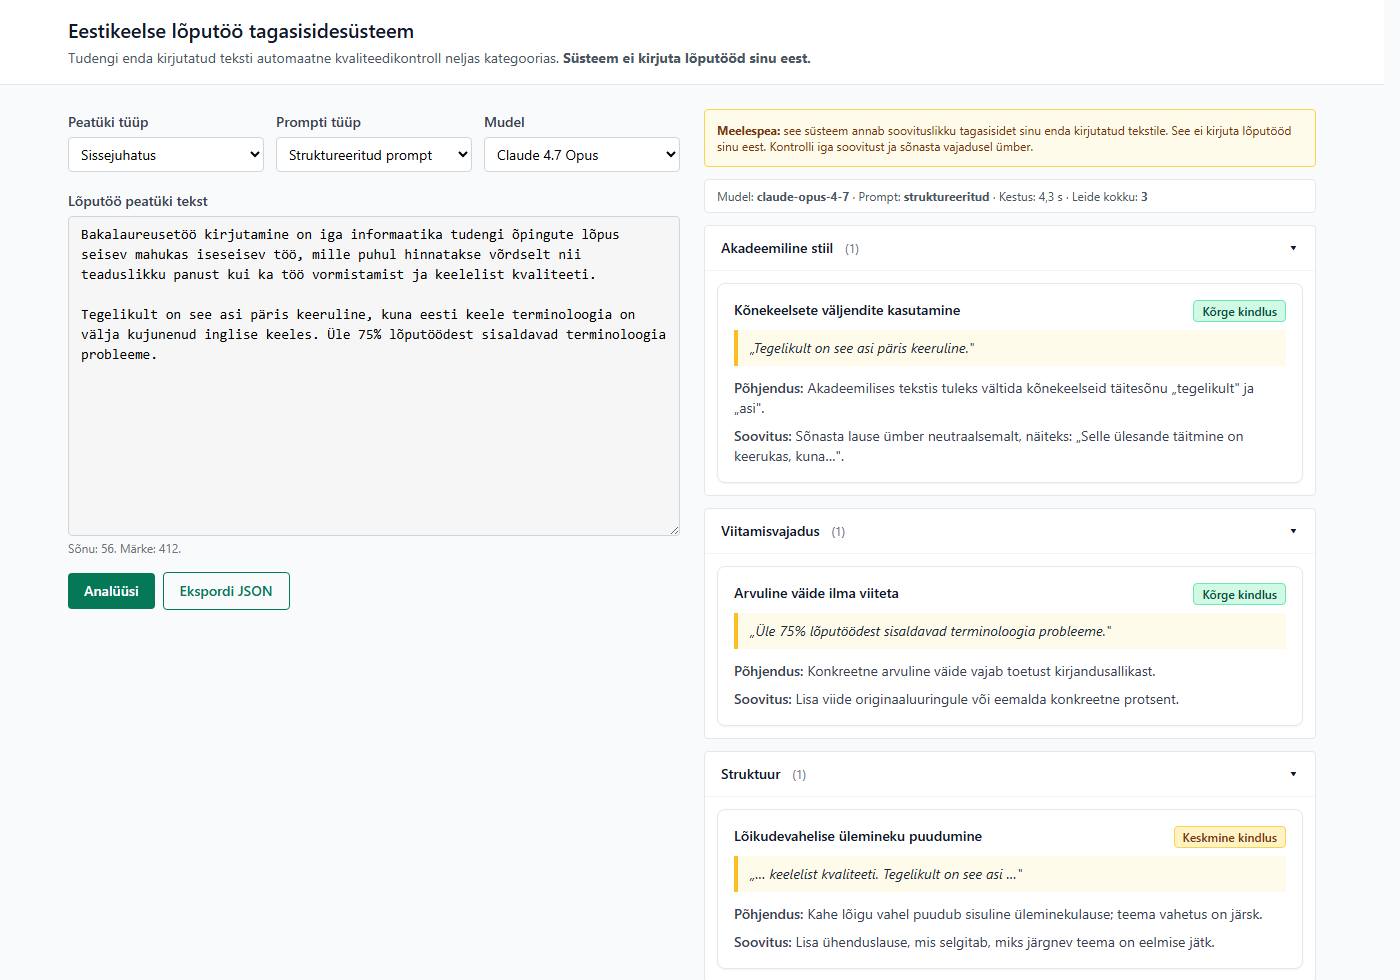
\includegraphics[width=\textwidth]{joonised/Joonis-Kasutajaliides.png}
    \caption{Prototüübi kasutajaliidese kuvatõmmis. Vasakul: tekstisisend ja konfiguratsioon (peatüki tüüp, prompti tüüp, mudel). Paremal: kategoriseeritud tagasiside, kus iga leid on kuvatud eraldi kaardina koos probleemse tsitaadi, kirjelduse, põhjenduse, soovituse ja kindlushinnanguga (kõrge — roheline, keskmine — kollane).}
    \label{fig:kasutajaliides}
\end{figure}

Kasutajaliidese disainivalikutest on olulisemad järgmised. \emph{Probleemse tsitaadi esiletõstmine} algses tekstis aitab kasutajal kohe leida tagasisides viidatud kohta. \emph{Kategooriate kokkupandavus} võimaldab kasutajal keskenduda ühele kategooriale korraga ning vältida visuaalset üleküllustamist juhul, kui leide on palju. \emph{Kindlushinnangu visuaalne kodeerimine} võimaldab kasutajal kiiresti otsustada, milliseid leide tasub esmalt kontrollida.

\subsection{Eetilised piirangud} \label{prototuup:eetika}

Süsteemi disainimisel on otseselt arvestatud sellega, et see ei muutuks tudengi jaoks teksti \emph{loomise} vahendiks. Selle tagamiseks rakendati neli eraldi meedet.

\textbf{Promptisisene piirang.} Süsteemi prompti algusesse on paigutatud selge nõue: \emph{Sul ei ole lubatud lõputööd tudengi eest kirjutada ega ümber sõnastada.} See vähendab oluliselt tõenäosust, et mudel pakub välja valmis ümbersõnastusi.

\textbf{Soovitus, mitte ümbersõnastus.} Tagasiside skeemis on \texttt{soovitus}-väli mõeldud lühikese juhise andmiseks (näiteks \emph{lisa enne alampealkirja sissejuhatav lõik, kus kirjeldad alampeatükkide loogilist järjekorda}), mitte tervete tekstilõikude valmis ümberkirjutamiseks. Backend lõikab \texttt{soovitus}-välja sisaldava teksti pikkuse 200 tähemärgini, mis muudab valmis ümberkirjutamise tehniliselt ebamugavaks.

\textbf{Selge teavitus kasutajaliidesest.} Igas vastuses on tagasiside paneeli päises pidevalt nähtav teade: \emph{See süsteem annab soovituslikku tagasisidet sinu enda kirjutatud tekstile. See ei kirjuta lõputööd sinu eest. Kontrolli iga soovitust ja sõnasta vajadusel ümber.}

\textbf{Privaatsus.} Demo-režiimis (vaikevalik) ei lahku kasutaja sisestatud tekst kohalikust masinast: backend tagastab salvestatud näidisvastuse. Kui kasutaja valib mudeliks Claude'i või GPT, saadetakse tekst LLM-i API-le ainult pärast seda, kui ta on kinnitanud konkreetses dialoogiaknas, et ta on sellest teadlik. Kohalik backend ei salvesta sisestatud teksti kettal; logitakse ainult anonüümne sündmus (näitajaid: prompti tüüp, peatüki tüüp, leidude arv kategooriate kaupa) hindamise jaoks.

Need meetmed ei ole täiuslikud – kasutaja võib endiselt prompti ümber sõnastada või luua ise ümber\-kirjutamise palve. Süsteemi roll on aga selgelt määratletud just tagasisidena, mitte loomise vahendina; vastutus konkreetse kasutusviisi eest jääb kasutajale.
